\documentclass[aspectratio=169,11pt]{beamer}

% --- Theme ---
\usetheme{metropolis}
\usepackage{appendixnumberbeamer}

% --- Packages ---
\usepackage{fontspec}
\usepackage{minted}
\setminted{fontsize=\small,breaklines=true}
\usepackage{booktabs}
\usepackage{tikz}
\usepackage{fontawesome5}

% --- Colors ---
\definecolor{healthgreen}{RGB}{34,139,34}
\definecolor{alertred}{RGB}{220,53,69}
\setbeamercolor{alerted text}{fg=alertred}

% --- Metadata ---
\title{Module 1: Python essentials for health professionals}
\subtitle{Data analysis with Python for health specialists}
\author{Ya\'{e} Ulrich Gaba}
\institute{AIRINA Labs}
\date{2026}

\begin{document}

% ============================================================
\maketitle

% ============================================================
\begin{frame}{Why are we here?}
\begin{columns}
\column{0.6\textwidth}
You are health professionals. You already know:
\begin{itemize}
  \item How to interpret lab values
  \item What a p-value means (roughly)
  \item That Excel has limits
\end{itemize}

\vspace{6pt}
Today you learn \alert{one new tool} that makes your existing skills more powerful.

\column{0.35\textwidth}
\centering
\Large
\faIcon{stethoscope} $\to$ \faIcon{python}\\[12pt]
{\small Clinical knowledge\\+ Python\\= reproducible research}
\end{columns}
\end{frame}

% ============================================================
\begin{frame}{Why Python, not Excel?}
\begin{table}
\begin{tabular}{lcc}
\toprule
& \textbf{Excel} & \textbf{Python} \\
\midrule
Reproducibility & \faIcon{times-circle} Click-based & \faIcon{check-circle} Script-based \\
Scale & Slow at 100K rows & Handles millions \\
Survival analysis & No & \texttt{lifelines} \\
Disease mapping & No & \texttt{geopandas} \\
ML prediction & No & \texttt{scikit-learn} \\
Cost & \$150/yr & Free \\
\bottomrule
\end{tabular}
\end{table}
\end{frame}

% ============================================================
\begin{frame}{Your workspace: Jupyter notebooks}
\centering
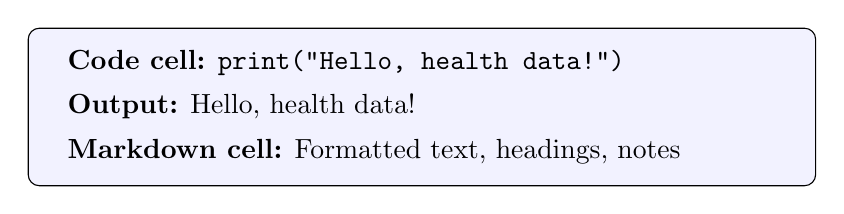
\begin{tikzpicture}
\node[draw,rounded corners,fill=blue!5,minimum width=10cm,minimum height=2cm] (nb) {
  \begin{minipage}{9cm}
  \textbf{Code cell:} \texttt{print("Hello, health data!")}\\[4pt]
  \textbf{Output:} Hello, health data!\\[4pt]
  \textbf{Markdown cell:} Formatted text, headings, notes
  \end{minipage}
};
\end{tikzpicture}

\vspace{8pt}
\faIcon{cloud} \textbf{Google Colab:} \url{colab.research.google.com} --- no installation needed\\
\faIcon{laptop} \textbf{Local:} Anaconda $\to$ Jupyter Notebook
\end{frame}

% ============================================================
\begin{frame}[fragile]{Variables: storing patient data}
\begin{minted}{python}
patient_age = 45              # int
temperature = 37.2            # float
diagnosis = "Type 2 Diabetes" # str
is_hospitalized = True        # bool
\end{minted}

\vspace{6pt}
\begin{alertblock}{Naming convention}
Use descriptive names: \texttt{patient\_age}, not \texttt{x}.
Your future self will thank you.
\end{alertblock}
\end{frame}

% ============================================================
\begin{frame}[fragile]{Collections: lists and dictionaries}
\begin{columns}
\column{0.48\textwidth}
\textbf{List} --- ordered values:
\begin{minted}{python}
bp = [120, 135, 128, 142]
print(bp[0])   # 120
print(len(bp)) # 4
\end{minted}

\column{0.48\textwidth}
\textbf{Dictionary} --- key-value pairs:
\begin{minted}{python}
patient = {
  "id": "PAT-42",
  "age": 58,
  "dx": "HTN",
}
print(patient["dx"])
\end{minted}
\end{columns}

\vspace{6pt}
Think of a dictionary as a \alert{patient chart} in code.
\end{frame}

% ============================================================
\begin{frame}[fragile]{Control flow: clinical classification}
\begin{minted}{python}
systolic = 148

if systolic >= 140:
    category = "Stage 2 Hypertension"
elif systolic >= 130:
    category = "Stage 1 Hypertension"
elif systolic >= 120:
    category = "Elevated"
else:
    category = "Normal"
\end{minted}

\vspace{4pt}
\textbf{Clinical mapping:} AHA/ACC 2017 guidelines $\to$ Python code.
\end{frame}

% ============================================================
\begin{frame}[fragile]{Loops: screening multiple patients}
\begin{minted}{python}
patients = [
  {"id": "P001", "hba1c": 5.4},
  {"id": "P002", "hba1c": 7.8},
  {"id": "P003", "hba1c": 6.1},
]

for p in patients:
    if p["hba1c"] >= 6.5:
        print(f"{p['id']}: Diabetic")
    elif p["hba1c"] >= 5.7:
        print(f"{p['id']}: Pre-diabetic")
    else:
        print(f"{p['id']}: Normal")
\end{minted}
\end{frame}

% ============================================================
\begin{frame}[fragile]{Functions: reusable calculations}
\begin{minted}{python}
def bmi(weight_kg, height_m):
    """Calculate Body Mass Index."""
    return weight_kg / (height_m ** 2)

def bmi_category(value):
    if value < 18.5: return "Underweight"
    elif value < 25:  return "Normal"
    elif value < 30:  return "Overweight"
    else:             return "Obese"

print(bmi(82, 1.75))  # 26.8
\end{minted}

\vspace{4pt}
Write once, use everywhere. \alert{Functions = reproducibility.}
\end{frame}

% ============================================================
\begin{frame}[fragile]{Importing libraries}
\begin{minted}{python}
import pandas as pd          # data tables
import numpy as np           # numbers
import matplotlib.pyplot as plt  # plots
import seaborn as sns        # statistical plots
from scipy import stats      # tests
\end{minted}

\vspace{6pt}
These five lines start \textbf{every} health data analysis notebook.

\vspace{6pt}
\begin{exampleblock}{Install if missing}
\texttt{pip install pandas matplotlib seaborn scipy}\\
In Colab: \texttt{!pip install lifelines}
\end{exampleblock}
\end{frame}

% ============================================================
\begin{frame}{What you can do after this module}
\begin{enumerate}
  \item Store patient data in Python variables, lists, and dictionaries
  \item Classify clinical measurements with \texttt{if/elif/else}
  \item Write reusable functions (BMI, eGFR, BP category)
  \item Loop through patient records for batch screening
  \item Import the core libraries for the rest of this course
\end{enumerate}

\vspace{12pt}
\centering
\Large \alert{Next: Module 2 --- Health data with Pandas}
\end{frame}

% ============================================================
\begin{frame}{Exercises (Hour 3)}
\begin{enumerate}
  \item \textbf{BP classifier:} Write \texttt{classify\_bp(systolic, diastolic)} returning AHA category
  \item \textbf{BMI batch:} Create 5 patient dicts with weight/height, compute and print BMI for each
  \item \textbf{eGFR function:} Implement the CKD-EPI equation
  \item \textbf{Mini-project:} Build a patient intake tool that prints a formatted clinical summary
\end{enumerate}
\end{frame}

\end{document}
